\documentclass[10pt, a4paper]{article}
\usepackage{lrec2014}
\usepackage{graphicx}
% for eps graphics

\usepackage{epstopdf}
\usepackage{url}
\usepackage{latexsym}

\usepackage{amsmath, amsthm, amssymb}
\usepackage{enumerate}
\usepackage[utf8]{inputenc}
\usepackage{arydshln} % the \hdashline and \cdashline commands which are the dashed counterparts of \hline and \cline

% citations

%% works
%\usepackage[authoryear]{natbib} %% should correspond to ACL 2013's \cite (author, year) vs. \shortcite (year)
%\usepackage[numbers]{natbib} %% should correspond to ACL 2013's \cite (author, year) vs. \shortcite (year)
%\newcommand{\citeparg}[2][]{\citep[#1]{#2}}

%% commands

\def\citep{\cite}
\def\citet{\newcite}

\newcommand{\todo}[1]{}
\newcommand{\onto}[1]{\texttt{\small #1}}
\newcommand{\word}[1]{\textsl{#1}}
\newcommand{\textem}[1]{\emph{#1}}
\newcommand{\tablesize}{\footnotesize}
\newcommand{\urly}{\tt}
\newcommand{\ign}[1]{}

%%%%%%%%%%%%%%%%%
% Anonymization %
%%%%%%%%%%%%%%%%%

%%%%%%%%%%%
% Content %
%%%%%%%%%%%

\title{Linked Data in Linguistics 2014. Introduction and Overview}

\name{Christian Chiarcos$^1$, John McCrae$^2$, Petya Osenova$^3$, Cristina Vertan$^4$}

\address{ $^1$ Goethe-Universität Frankfurt am Main, Germany, \url{chiarcos@uni-frankfurt.de}\\
		  $^2$ Universität Bielefeld, Germany, \url{jmcrae@cit-ec.uni-bielefeld.de}\\
		  $^3$ University of Sofia, Bulgaria, \url{petya@bultreebank.org}\\ 
		  $^4$ Universität Hamburg, Germany,\url{cristina.vertan@uni-hamburg.de}
		  \\}

\begin{abstract}
	The Linked Data in Linguistics (LDL) workshop series brings together researchers from various fields of linguistics, natural language processing, and information technology to present and discuss principles, case studies, and best practices for representing, publishing and linking linguistic data collections. A  major outcome of our work is the Linguistic Linked Open Data (LLOD) cloud, an LOD (sub-)cloud of linguistic resources, which covers various linguistic data bases, lexicons, corpora, terminology and metadata repositories.\\
%	
	As a general introduction into the topic, we describe the concept of Linked Data, its application in linguistics and the Linguistic Linked Open Data (LLOD) cloud, its history, and in particular, community activities since the last LDL workshop at LREC-2014. In addition, we present the contributions of LDL-2015 as well as the newly compiled LLOD cloud diagram. \\
%	
	The fourth instantiation of this series, collocated with ACL-IJCNLP 2015, the 53rd Annual Meeting of the Association of Computational Linguistics and the 7th Joint Conference on Natural Language Processing of the Asian Federation of Natural Language Processing, July 31st, 2015, in Beijing, China, is specifically dedicated to Resources and Applications. With the rapid development of the LLOD cloud in last years, and the recent surge of interest in Linked Data in (Computational) Linguistics, the focus of our community is increasingly shifting towards applications of this data, especially -- but not limited to -- Natural Language Processing. 
	Nevertheless, contributions with respect to any application of Linked Data to linguistically and/or NLP-relevant resources are welcome, as well.

%% not in ACL-2015 style
% \Keywords{Linked Data in Linguistics (LDL), Linguistic Linked Open Data (LLOD) cloud}

\end{abstract}

\begin{document}

\maketitleabstract

\section{Background and Motivation}
\label{sec-background}

After
half a century of computational linguistics \citep{dostert1955georgetown},               % Georgetown experiment (1954)
quantitative typology \citep{greenberg60-quant},
empirical, corpus-based study of language \citep{francis-kucera1964},  and % Kucera & Francis (1961/63), Brown corpus
computational lexicography \citep{morris1969},
researchers in computational linguistics, natural language processing (NLP) or information technology, as well as in Digital Humanities,
 are confronted with an immense wealth of linguistic resources, that are not only growing in number, but also in their heterogeneity.
Accordingly, the limited interoperability between linguistic resources has been recognized as a major obstacle for data use and 
re-use within and across discipline boundaries, and represents one of the prime motivations for adopting Linked Data to our field. 
 
Interoperability involves two aspects \citep{ide-pustejovsky2010-interoperability}:

\smallskip
\noindent
\paragraph{(a) How to access a resource?} (Structural interoperability)
Resources use comparable formalisms to represent and to access data (formats, protocols, query languages, etc.), so that they can be accessed in a uniform way and that their information can be integrated with each other.

\smallskip
\noindent
\paragraph{(b) How to interpret information from a resource?} ({Conceptual} interoperability)
Resources share a common vocabulary, so that linguistic information from one resource can be resolved against information from another resource, e.g., grammatical descriptions can be linked to a terminology repository.

\bigskip

\noindent With the rise of the Semantic Web, new representation formalisms and novel technologies have become available, and different communities are becoming increasingly aware of the potential of these developments with respect to the challenges posited by the heterogeneity and multitude of linguistic resources available today. Many of these approaches follow the \textbf{Linked (Open) Data paradigm} \citep{bernersLee2006_linkeddata}, and this line of research, and its application to resources relevant for linguistics and/or NLP represent the focus of our work.

\subsection{Linked Data}

The Linked Open Data paradigm postulates four rules for the publication and representation of Web resources:
(1) Referred entities should be designated by using URIs,
(2) these URIs should be resolvable over HTTP,
(3) data should be represented by means of W3C standards (such as RDF),
(4) and a resource should include links to other resources.
These rules facilitate information integration, and thus, interoperability, in that they require that entities can be addressed in a globally unambiguous way (1), that they can be accessed (2) and interpreted (3), and that entities that are associated on a conceptual level are also physically associated with each other (4).

In the definition of Linked Data, the \textbf{Resource Description Framework (RDF)} receives special attention. \index{RDF (Resource Description Framework)}RDF was designed to provide metadata about resources that are available either offline (e.g., books in a library) or online (e.g., eBooks in a store). \index{RDF (Resource Description Framework)}RDF provides a generic data model based on labeled directed %(multi-)
graphs, which can be serialized in different formats. Information is expressed in terms of \emph{triples} - consisting of a \emph{property} (relation, i.e., a labeled edge) that connects a \emph{subject} (a resource, i.e., a labeled node) with its \emph{object} (another resource, or a literal, e.g., a string).
RDF resources (nodes)\footnote{
    The term `resource' is ambiguous: \emph{Linguistic} resources are structured collections of data which can be represented, for example, in RDF. In RDF, however, `resource' is the conventional name of a node in the graph, because, historically, these nodes were meant to represent objects that are described by metadata. We use the terms `node' or `concept' whenever \emph{RDF} resources are meant in ambiguous cases.
} are represented by \emph{Uniform Resource Identifiers (URIs)}. They are thus globally unambiguous in the web of data. This allows resources hosted at different locations to refer to each other, and thereby to create a network of data collections whose elements are densely interwoven.

Several data base implementations for \index{RDF (Resource Description Framework)}RDF data are available, and these can be accessed using \textbf{SPARQL} \citep{prud2008sparql}, a standardized query language for \index{RDF (Resource Description Framework)}RDF data.
SPARQL uses a triple notation similar to RDF, only that properties and \index{RDF (Resource Description Framework)}RDF resources can be replaced by variables. SPARQL is inspired by SQL, variables can be introduced in a separate \onto{SELECT} block, and constraints on these variables are expressed in a \onto{WHERE} block in a triple notation. SPARQL does not only support running queries against individual \index{RDF (Resource Description Framework)}RDF data bases that are accessible over HTTP (so-called `SPARQL end points'), but also, it allows us to combine information from multiple repositories (federation). \index{RDF (Resource Description Framework)}RDF can thus not only be used to \emph{establish} a network, or cloud, of data collections, but also, to \emph{query} this network directly.

RDF has been applied for various purposes beyond its original field of application. In particular, it evolved into a generic format for knowledge representation. It was readily adopted by disciplines as different as biomedicine and bibliography, and eventually it became one of the building stones of the \textbf{Semantic Web}. Due to its application across discipline boundaries, \index{RDF (Resource Description Framework)}RDF is maintained by a large and active community of users and developers, and it comes with a rich infrastructure of APIs, tools, databases, query languages, and multiple sub-languages that have been developed to define data structures that are more specialized than the graphs represented by RDF. These sub-languages can be used to create \emph{reserved vocabularies} and \emph{structural constraints} for \index{RDF (Resource Description Framework)}RDF data. For example, the Web Ontology Language (OWL) defines the datatypes necessary for the representation of ontologies as an extension of RDF, i.e., \emph{classes} (concepts), \emph{instances} (individuals) and \emph{properties} (relations). 
%OWL/DL is an OWL dialect that is restricted such that the language corresponds to a description logic, i.e., a decidable fragment of first-order predicate logic. Exploiting this restriction, a number of reasoners have been developed that allow the verification of consistency constraints (\emph{axioms}) as well as methods  to draw inferences from logical relations in the ontology. If modeled as ontologies, the semantic consistency of linguistic resources can be validated and implicit information can be inferred.

The concept of Linked Data is closely coupled with the idea of \textbf{openness} (otherwise, the linking is only partially reproducible), and in 2010, the original definition of Linked Open Data has been extended with a 5 star rating system for data on the Web.\footnote{\url{http://www.w3.org/DesignIssues/LinkedData.html}, paragraph `Is your Linked Open Data 5 Star?'} The first star is achieved by publishing data on the Web (in any format) under an open license, and the second, third and fourth star require machine-readable data, a non-proprietary format, and using standards like RDF, respectively. The fifth star is achieved by linking the data to other people's data to provide context.
If (linguistic) resources are published in accordance with these rules, it is possible to follow links between existing resources to find other, related data and exploit network effects.

\subsection{Linked Data for Linguistics and NLP}
\label{sec-linked-data}

Publishing Linked Data allows resources to be globally and uniquely identified such that they can be retrieved through standard Web protocols. Moreover, resources can be easily linked to one another in a uniform fashion and thus become structurally interoperable. \citet{chiarcos-etal2012-ntrolr} identified five main benefits of Linked Data for Linguistics and NLP: 

\noindent
\paragraph{(1) Conceptual Interoperability}
Semantic Web technologies allow to provide, to maintain and to share centralized, but freely accessible terminology repositories. 
Reference to such terminology repositories facilitates conceptual interoperability as different concepts used in the annotation are backed up by externally provided definitions, and these common definitions may be employed for comparison or information integration across heterogeneous resources.

\smallskip\noindent
\paragraph{(2) Linking through URIs}
URIs provide globally unambiguous identifiers, and if resources are accessible over HTTP, it is possible to create resolvable references to URIs. Different resources developed by independent research groups can be connected into a cloud of resources.

\smallskip\noindent
\paragraph{(3) Information Integration at Query Runtime (Federation)}
Along with HTTP-accessible repositories and resolvable URIs, it is possible to combine information from physically separated  repositories in a single query at runtime: 
Resources can be uniquely identified and easily referenced from any other resource on the Web through URIs. 
Similar to hyperlinks in the HTML web, the web of data created by these links allows to navigate along these connections, 
and thereby to freely integrate information from different resources in the cloud.

\smallskip\noindent
\paragraph{(4) Dynamic Import}
When linguistic resources are interlinked by references to resolvable URIs instead of system-defined IDs (or static copies of parts from another resource), we always provide access to the most recent version of a resource. 
For community-maintained terminology repositories like the ISO TC37/SC4 Data Category Registry \citep[ISOcat]{wright2004global,windhouwer-wright2012}, for example, new categories, definitions or examples can be introduced occasionally, and this information is available immediately to anyone whose resources refer to ISOcat URIs. 
In order to preserve link consistency among Linguistic Linked Open Data resources, however, it is strongly advised to apply a proper versioning system such that backward-compatibility can be preserved: Adding concepts or examples is unproblematic, but when concepts are deleted, renamed or redefined, a new version should be provided.

\smallskip\noindent
\paragraph{(5) Ecosystem}
RDF as a data exchange framework is maintained by an interdisciplinary, large and active community, and it comes with a developed infrastructure that provides APIs, database implementations, technical support and va\-li\-da\-tors for various RDF-based languages, e.g., reasoners for OWL. For developers of linguistic resources, this ecosystem can provide technological support or off-the-shelf implementations for common problems, e.g., the de\-ve\-lop\-ment of a database that is capable of support flexible, graph-based data structures as necessary for multi-layer corpora \citep{ide-suderman07-graf}.

\smallskip\noindent
\paragraph{(6) Distributed Development}
To these, \citet{chiarcos-etal-2013-ldl-intro} add that the distributed approach of the Linked Data paradigm facilitates the distributed de\-ve\-lop\-ment of a web of resources and collaboration between researchers that provide and use this data and that employ a shared set of technologies. One consequence is the emergence of interdisciplinary efforts to create large and interconnected sets of resources in linguistics and beyond. The LDL workshop series provides a forum to discuss and to facilitate such on-going developments, in particular, the emerging Linguistic Linked Open Data cloud.
\section{Linguistic Linked Open Data: Building the Cloud}

Recent years have seen not only a number of approaches to provide linguistic data as Linked Data, but also the emergence of larger initiatives that aim at interconnecting these resources.
Among these, the Open Linguistics Working Group (OWLG) of the Open Knowledge Foundation (OKFN) has spearheaded the creation of 
new data and the republishing of existing linguistic resources as part of the emerging Linguistic Linked Open Data (LLOD) cloud. 
As the OWLG organizes the LDL workshop series as a vehicle to facilitate this process, we would like to take the chance to unveil the revised cloud diagram on the occasion of LDL-2014.

\subsection{The LLOD Cloud}

In our current, informal understanding, \textbf{Linguistic Data} is pragmatically defined as any kind of resource considered relevant for linguistic research or Natural Language Processing tasks. 
Our assessment of relevance follows the classification of resources provided by data providers or the community, as reflected, for example, in tags assigned to resources at \url{datahub.io}, the meta data repository from which the LLOD cloud is currently being built. During diagram compilation, ressources associated with the OWLG, or with tags like `LLOD', `linguistics', etc. are gathered, stored in a JSON document, categorized according to manually defined classification rules, and plotted and reformatted using a GraphML editor.\footnote{
	The extraction scripts can be found under \url{https://github.com/jmccrae/llod-cloud.py}.
}

Among these data sets, we encourage the use of \textbf{open} licenses and limit the diagram to such data sets. As defined by the Open Definition, ``openness'' refers to ``[any] piece of content or data [that] is open if anyone is free to use, reuse, and redistribute it -- subject only, at most, to the requirement to attribute and share-alike.''\footnote{\url{http://opendefinition.org}}

Linguistic \textbf{Linked} Open Data, then, comprises resources that are provided under an open license and published in conformance with the Linked Data principles as stated above.
Typically, these do not represent resources which are RDF-native, but resources that have been transformed into Linked Data. 

This also has an impact on the types of linguistic resources considered here, in particular the concept of \textbf{corpora}:
In empirical linguistics and NLP, \emph{collections of primary data} represent the elementary foundation of research and development. 
Yet, while it is possible to represent primary data such as plain text in RDF, this is not necessarily the most efficient way of doing so -- also given the fact that specialized XML-based standards such as the Text Encoding Iniative\footnote{
	\url{http://www.tei-c.org}
}
are well-established and widely used.
However, RDF provides highly flexible data structures that can be employed to represent linguistic annotations of arbitrary complexity. 
As understood \emph{here}, a `corpus' is thus always a linguistically analyzed resource:
Along with classical representations where both annotations \emph{and} primary data are modeled in RDF (e.g., in the seminal study of \citep{burchardt2008formalising}), 
but also hybrid data sets where only annotations are provided as Linked Data, but the primary data is stored in a conventional format (e.g., \citep{cassidy2010rdf}).
At the moment, corpora in the LLOD cloud seem to be relatively rare (see `CORPUS' resources in Fig.\ \ref{figI18nLOD}), 
but this only reflects the fact that several corpora had to be excluded from the diagram because they were not linked yet with other LLOD data sets such as lexical resources or repositories of annotation terminology.

Beyond representing linguistic analyses for collections of examples, text fragments, or entire discourses, 
the Linked Data paradigm particularly facilitates the management of \textbf{information about language and language resources} (`METADATA' in Fig.\ \ref{figI18nLOD}, \textsc{language\_description}).
These include linguistic databases (collections of features and inventories of individual languages, e.g., from linguistic typology), repositories of linguistic terminology (e.g., grammatical categories or language identifiers), and metadata about language resources (incl. bibliographical data).
While bibliographical data and terminology management represent classical Linked Data applications, our \emph{databases} are a specifically linguistic resource:
Databases of features of individual languages are a particularly heterogeneous group of linguistic resources; they contain complex and manifold types of information, e.g., feature structures that represent typologically relevant phenomena, along with examples for their illustration and annotations (glosses) and translations applied to these examples (structurally comparable to corpus data), or word lists (structurally comparable to lexical-semantic resources). RDF as a generic representation formalism is thus particularly appealing for this class of resources.

The third major group of resources in the diagram are \textbf{lexical-semantic resources} (`LEXICON', \ref{figI18nLOD}), i.e., resources focusing on the general meaning of words and the structure of semantic concepts. 
These represent by far the most established type of linguistic resources in the LD context: They have been of inherent interest to the Semantic Web community, and hence a long tradition in this regard, going back to earliest attempts to integrate WordNet into the SW world \citep{gangemi2003ontowordnet}. 
In the diagram, we distinguish two types of lexical-semantic resources, i.e., \emph{lexical resources} in a strict sense (which provide specifically linguistic information, e.g., grammatical features, as found, e.g., in a dictionary, or in a WordNet), and and \emph{general knowledge bases} (such as classical thesauri or semantic repositories such as YAGO and DBpedia) 
whose origins lay outside of the stricter boundaries of linguistics or NLP. 
While the latter do not provide us with grammatical information, they formalize semantic knowledge, and in this respect, they are of immanent relevance for Natural Language Processing tasks such as Named Entity Recognition or Anaphora Resolution. 

\begin{figure*}[t]
 \begin{center}
% \includegraphics[width=0.97\textwidth]{images/LODLinguistics.jpg}
% \includegraphics[width=0.97\textwidth]{images/llod}
 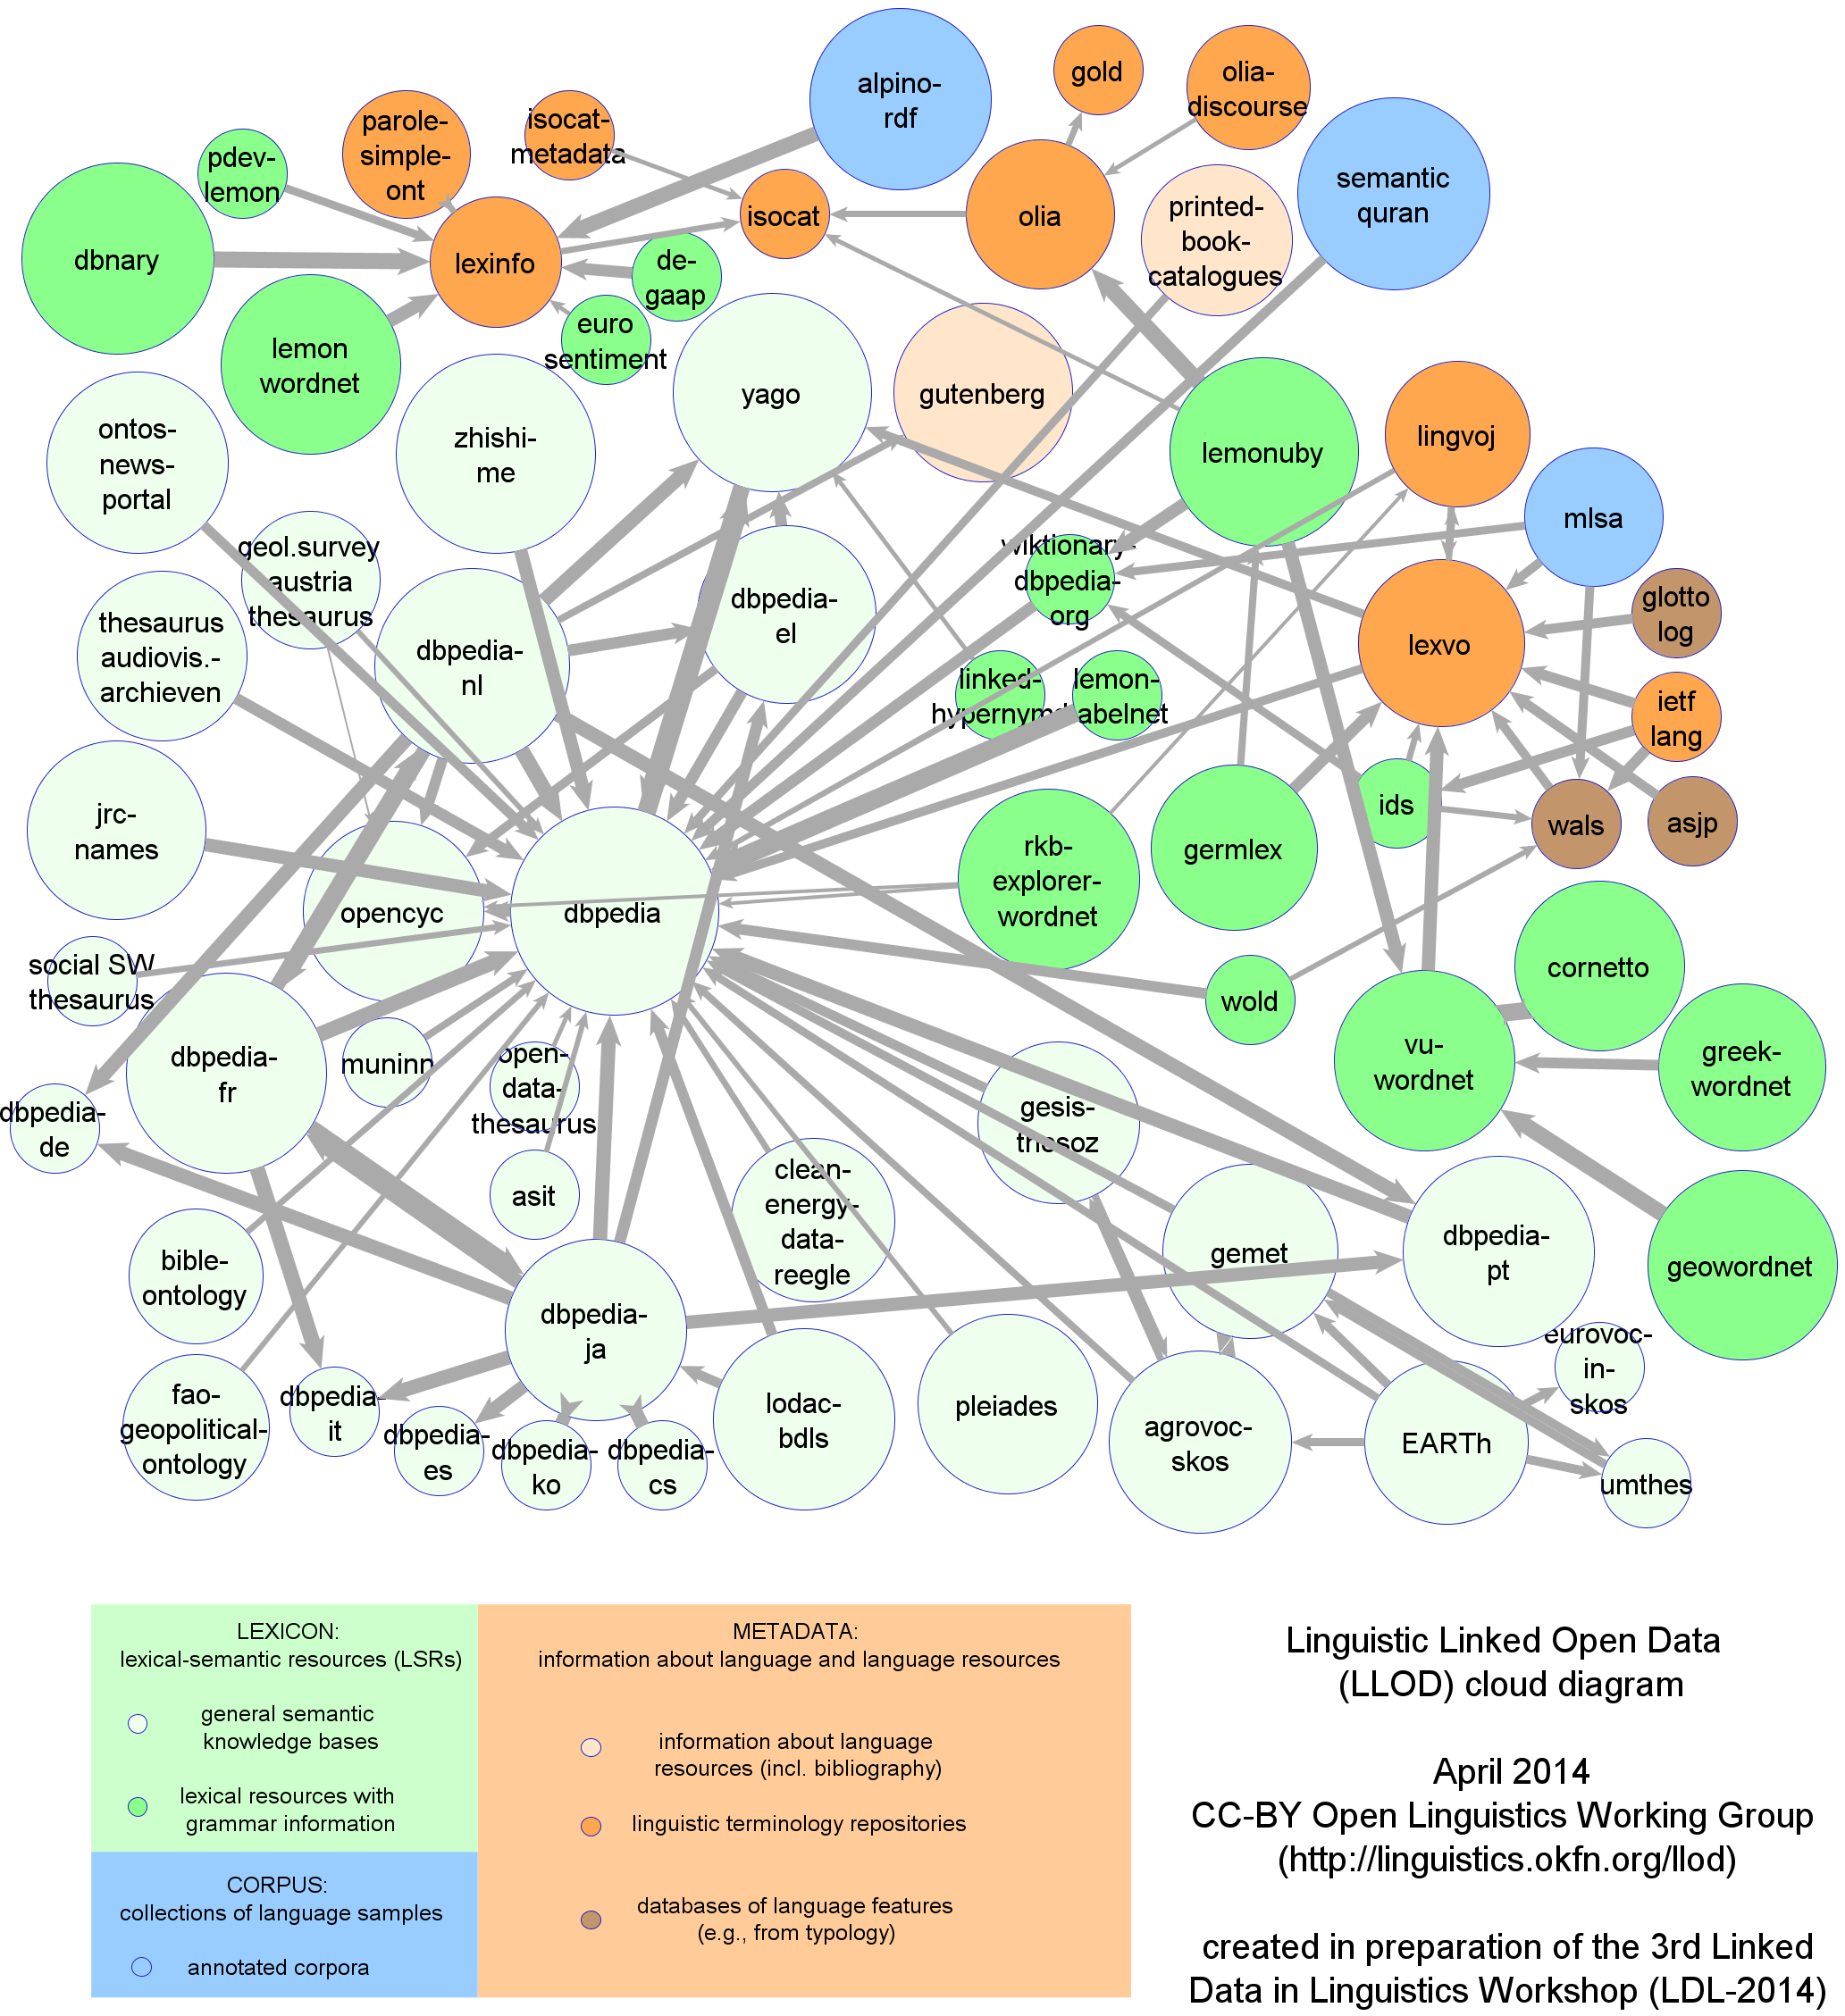
\includegraphics[width=0.8\textwidth]{llod-colored.png}
 \end{center}
\caption{Linguistic Linked Open Data cloud as of September 2013.}
\label{figI18nLOD}
\end{figure*}

\subsection{Recent Developments}

Since the publication of the last LLOD cloud diagram at LDL-2013, Sep 2013 in Italy, Pisa, we have continued to gather and to convert data sets, to refine our classification of language resources and encouraged others to contribute, e.g., by organizing LDL-2014 and the associated data challenge (see below).

These efforts have met with success such that the number of candidate resources for the cloud has increased substantially, from 65 resources in September 2013 to 107 in April 2014. 
We thus enforced the constraints imposed on resources in the cloud diagram. As of April 2014, we limit datasets in the cloud diagram to those with links to other LLOD data sets. 
Applying these stricter filters, we arrive at 68 resources in the new diagram.
For generating the diagram, we rely on the metadata as provided by Datahub.io, so only datasets are considered whose links with other LLOD data sets are explicitly documented there.
During diagram generation, we test whether the URLs given for the data are responding. At the moment, we do not, however, validate the information provided there, but a stricter validation routine is envisioned. 

Among others, novel data sets include resources prepared for LDL-2014 and the data challenge, but also resources that have not been covered by earlier diagram instantiations because they lacked the necessary tags to recognize them as being linguistically relevant. An example for the latter is the the Greek WordNet, whose RDF edition has been released in early 2013,\footnote{
	\url{http://datahub.io/de/dataset/greek-wordnet}, see \url{http://okfn.gr/2013/01/983/} for a description.
}
but also, several thesauri and multilingual vocabularies.
This provides a partial explanation for the growth of the cloud particular with respect to lexical resources. 

At the same time, the growing number of linked lexical resources also reflects the activities of the W3C Ontology-Lexica Community Group (OntoLex). The OntoLex group is not only closely collaborating with the OWLG, but both also have a considerable overlap in terms of their members, and as for LDL-2013, several LDL-2014 organizers are active in both groups.
While the OWLG is interested in open linguistic resources in general, the OntoLex group takes a specific focus on lexical resources, culminating in the proposal of a common model for machine-readable lexicons in RDF, the \emph{lemon} model \cite{mccrae2012integrating}. 
By now, already 41\% of lexical resources (7 out of 17) in the diagram (lemonWordNet, PDEVlemon, Parole/Simple, lemonUby, lemonBabelNet, germlex, DBnary) employ \emph{lemon} or \emph{lemon}-derived vocabularies, so that we see a considerable degree of convergence in this field. 
The resulting degree of interoperability and visibility arising from the use of shared vocabularies is certainly one of the most concrete achievements of the community activities we aimed to initiate with forming the OWLG, preparing the LLOD diagram and conducting workshops at linguistic, NLP and IT conferences.

\subsection{Behind LDL-2014}

% The LDL workshop series and LDL-2014 are organized by the Open Linguistics Working Group, and supported by LIDER & QTLeap

% An important vehicle for this process are workshops organized by the OWLG. 
% These include the Linked Data in Linguistics workshop series (March 2012 in Frankfurt am Main, Germany; Sep 2013 in Pisa, Italy; May 2014 in Reykjavik, Iceland) which bring together researchers from linguistics, NLP and Semantic Web, 
% as well as more specialized events such as a workshop on Multilingual Linked Open Data for Enterprises (MLODE-2012: Sep 2012 in Leipzig, Germany) or the 
% theme session on Linked Data in Linguistic Typology (at the 10th Biennial Conference of the Association for Linguistic Typology, ALT-2013, Aug 2013 in Leipzig, Germany), as well as presentations, panels and informal meetings at selected conferences.

% Yet, before giving an overview over the contributions to LDL-2014, 
% Related initiatives include the W3C Ontology-Lexica Community Group that is seeking to develop standard models for representing and publishing (ontology-) lexica and other lexical resources as RDF, and th


% Since LDL-2013, the  


% The LDL workshop series is organized by the 

% , culminating on the creation of a Linguistic Linked Open Data (LLOD) cloud, i.e., a Linked Open Data (sub-)cloud of linguistic resources.



% The 

% LDL-2013 is organized in the context of two recent community efforts, the Open Linguistics Working Group  (OWLG), and the W3C Ontology-Lexica Community Group (OntoLex). 


The LLOD cloud is a result of a coordinated effort of the {\bf Open Linguistics Working Group (OWLG)},\footnote{\url{http://linguistics.okfn.org}} a network open to anyone interested in linguistic resources and/or the publication of these under an open license. The OWLG is a working group of the Open Knowledge Foundation (OKFN),\footnote{\url{http://okfn.org/}} a community-based non-profit organization promoting open knowledge (i.e., data and content that is free to use, re-use and to be distributed without restriction).
%The OWLG adopts OKFN's principles, definitions and infrastructure as far as they are relevant for linguistic data. The OKFN defines standards and develops tools that allow anyone to create, discover and share open data. The Open Definition of the OKFN states that ``openness'' refers to: ``A piece of content or data [that] is open if anyone is free to use, reuse, and redistribute it -- subject only, at most, to the requirement to attribute and share-alike.''\footnote{\url{http://opendefinition.org}}
%The Open Definition is accompanied by a list of compliant licenses.
%One important aspect here is that openness should not constrain the use of data provided under these licenses, e.g., its commercial use, and that it should allow to complement these with proprietary resources. Adopting this understanding of openness for the LLOD cloud warantees that the resources contained in the cloud are available under \emph{any circumstances}.

%One tool that the OKFN provides is \textbf{CKAN},\footnote{\url{http://ckan.org/}} a catalog system for open data sets. CKAN is an open-source data portal software developed to easily publish, find and reuse open content and data, particularly in ways that are also machine automatable. The OKFN also hosts various working groups addressing problems of open data in different domains. Currently, there are 18 OKFN \textbf{working groups} covering fields as diverse as government data, economics, archeology, text books and cultural heritage. The OKFN organizes various events, such as the Open Knowledge Conference (OKCon), and facilitates the exchange of ideas between different working groups. The vision of the OKFN is a world in which open knowledge is ubiquitous. In this paper, we apply the aims of open knowledge to data in the field of linguistics.

Since its formation in 2010, the Open Linguistics Working Group has grown steadily. One of our primary goals is to attain openness in linguistics through:

\begin{enumerate}
\item Promoting the idea of open linguistic resources,
\item Developing the means for the representation of open data, and
\item Encouraging the exchange of ideas across different disciplines.
\end{enumerate}

\noindent 
%Publishing linguistic data under open licenses is an important issue in academic research, as well as in the de\-ve\-lop\-ment of applications. We see increasing support for this in the linguistics community \citep{Pederson:2008}, and there are a growing number of resources published under open licenses \citep{meyers2007shared}. There are many reasons for publishing resources under open licenses: for instance, freely available data can be more easily re-used, double investments can be avoided, and results can be replicated. Also, other researchers can build on this data, and subsequently refer to the publications associated with it. Nevertheless, a number of ethical, legal and sociological problems are associated with open data,\footnote{
%For example, complex copyright situations may arise if one resource (say, a lexicon) was developed on the basis of another resource (say, a newspaper archive), and researchers are uncertain whether the examples from the original newspaper contained in the lexicon violate the original copyright. Ethical problems may arise if a data base of quotations from a newspaper is linked to a data base of speakers, and this data base is further connected with, say, obituaries from the same newspaper. Even if this was done only in order to study generation-specific language variation, one may wonder whether such a accumulation of information violates the privacy of the people involved.
%}
%and the technologies that establish interoperability (and thus, re-usability) of linguistic resources are still under de\-ve\-lop\-ment. 
%
The OWLG represents an open forum for interested individuals to address these and related issues.
At the time of writing, the group consists of about 100 people from 20 different countries.
Our group is relatively small, but continuously growing and sufficiently heterogeneous. It includes
people from library science, typology, historical linguistics, cognitive science, computational linguistics, and information technology; the ground for fruitful interdisciplinary discussions has been laid out.
One concrete result emerging out of collaborations between a large number of OWLG members is the LLOD cloud as already sketched above.
%Independent research activities of many community members involve the application of RDF/OWL to represent linguistic corpora, lexical-semantic resources, terminology repositories and metadata collections about linguistic data collections and publications, and to many of them, the Linked Open Data paradigm represents a particularly appealing set of technologies. Within the OWLG, these activities converged towards building the cloud. 

The emergence of the LLOD cloud out of a set of isolated resources was accompanied and facilitated by a series of \textbf{workshops and publications} organized under the umbrella of the OWLG, including the Open Linguistics track at the Open Knowledge Conference (OKCon-2010, July 2010, Berlin, Germany), the First Workshop on Linked Data in Linguistics (LDL-2012, March 2012, Frankfurt am Main, Germany), the Workshop on Multilingual Linked Open Data for Enterprises (MLODE-2012, September 2012, Leipzig, Germany), the Linked Data for Linguistic Typology track at ALT-2012 (September 2013, Leipzig, Germany). Plans to create a LLOD cloud were first publicly announced at LDL-2012, and subsequently, a first instance of the LLOD materialized as a result of the MLODE-2012 workshop, its accompanying hackathon and the data postproceedings that will appear as a special issue of the Semantic Web Journal (SWJ). The Second Workshop on Linked Data in Linguistics (LDL-2013) continues this series of workshops. In order to further contribute to the integration of the field, it is organized as a joint event of the OWLG and the W3C Ontology-Lexica Community Group.

The \textbf{Ontology-Lexica Community (OntoLex) Group}\footnote{\url{http://www.w3.org/community/ontolex}} was founded  in September 2011 as a W3C Community and Business Group. It aims to produce specifications for a lexicon-ontology model that can be used to provide rich linguistic grounding for domain ontologies.
Rich linguistic grounding include the representation of morphological, syntactic properties of lexical entries as well as the syntax-semantics interface, i.e., the meaning of these lexical entries with respect to the ontology in question. An important issue herein will be to clarify how extant lexical and language resources can be leveraged and reused for this purpose. As a byproduct of this work on specifying a lexicon-ontology model, it is hoped that such a model can become the basis for a web of lexical linked data: a network of lexical and terminological resources that are linked according to the Linked Data Principles forming a large network of lexico-syntactic knowledge.

The OntoLex W3C Community Group has been working for more than a year on realizing a proposal for a standard ontology lexicon model, currently discussed under the the designation \emph{lemon}. As the core specification of the model is almost complete, the group started to develop of additional modules for specific tasks and use cases, and some of these are presented at LDL-2013.


\section{LDL-2014: The 3rd Workshop on Linked Data in Linguistics}

For the 3rd edition of the workshop on Linked Data in Linguistics, we invited contributions discussing the application of the Linked Open Data paradigm to linguistic data in various fields of linguistics, natural language processing, knowledge management and information technology in order to to present and discuss \emph{principles}, \emph{case studies}, and \emph{best practices} for representing, publishing and linking mono- and multilingual linguistic and knowledge data collections, including corpora, grammars, dictionaries, wordnets, translation memories, domain specific ontologies etc. 

In this regard, the Linked Data paradigm might provide an important step towards making linguistic data: i) easily and uniformly queryable, ii) interoperable and iii) sharable over the Web using open standards such as the HTTP protocol and the RDF data model. The adaptation of some processes and best practices to \textbf{multilingual linguistic resources and knowledge bases} acquires special relevance in this context. Some processes may need to be modified to accommodate the publication of resources that contain information in several languages. Also the linking process between linguistic resources in different languages poses important research questions, as well as the development and application of freely available knowledge bases and crowdsourcing to compensate the lack of publicly accessible language resources for various languages.

Further, LDL-2014 provides a forum for researchers on natural language processing and semantic web technologies to present case studies and best practices on the exploitation of linguistic resources exposed on the Web for \textbf{Natural Language Processing} applications, or other content-centered applications such as content analytics, knowledge extraction, etc. The availability of massive linked open knowledge resources raises the question how such data can be suitably employed to facilitate different NLP tasks and research questions. Following the tradition of earlier LDL workshops, we encouraged contributions to the Linguistic Linked Open Data (LLOD) cloud and research on this basis. In particular, this pertains to contributions that demonstrate an added value resulting from the combination of linked datasets and ontologies as a source for semantic information with linguistic resources published according to as linked data principles. Another important question to be addressed in the workshop is how Natural Language Processing techniques can be employed to further facilitate the growth and enrichment of linguistic resources on the Web.

The call for papers emphasized the following topics of interest:

\begin{enumerate}
\item \textbf{Use cases} and project proposals for the creation, publication or application of linguistic data collections that are linked with other resources
\item \textbf{Modelling} linguistic data and metadata with OWL and/or RDF
\item \textbf{Ontologies} for linguistic data and metadata collections as well as cross-lingual retrieval
\item Description of \textbf{data sets} following Linked Data principles
\item \textbf{Applications of such data}, other ontologies or linked data from any subdiscipline of linguistics % (may include work in progress or project descriptions)
\item \textbf{NLP\&LOD}: Application and applicability of (Linguistic) Linked Open Data in NLP / NLP contributions to (Linguistic) Linked Open Data
\item Challenges of \textbf{multilinguality} and \textbf{collaboratively constructed open resources} % and the use of LOD %and collaboratively constructed open resources 
for knowledge extraction, machine translation and other NLP tasks.
\item \textbf{Legal and social aspects} of Linguistic Linked Open Data
\item \textbf{Best practices} for the publication and linking of multilingual knowledge resources
\end{enumerate}

\noindent 
Along with regular workshop submissions, we invited contributions to the associated data challenge (see below) for data sets together with data set descriptions.
In total, we received 19 submissions in response to our calls, including 5 data set descriptions for the associated data challenge. Regular submissions were reviewed by at least 3 
% actually 4, IMHO
members of the program committee. 
On the basis of these reviews, we decided to accept 6 papers as full papers and 4 as short papers.

The 10 accepted papers address a wide range of problems in the area of NLP and (Linguistic) Linked Open Data, pertaining to modeling, representation, analysis and publishing of various 
data or metadata.

Taxken together, the contributions cover a vast and heterogeneous field, they involve different types of lexical resources, such as etymological, diachronic, web, movies, and grammar terminology, but also issues of localization and multilinguality. Our tentative classification, which we follow in both the proceedings and the remainder of this section, is a compromise between a classification on grounds of resource types and prospective applications:

A particularly popular branch of research is concerned with \textbf{modeling lexical-semantic resources} using RDF-based vocabularies and lexicon-to-ontology mappings, most noteably \emph{lemon}. 
This group of submissions partially overlaps with a surprisingly large number of papers concerned with the modeling of multilingual resources in more academic fields of linguistics, namely \textbf{cross-linguistic studies} in linguistic typology and comparative linguistics.
A third group of papers involves different conceptions of \textbf{metadata}, i.e., terminology for linguistic categories and language resources, but also annotations to multimedial content.
Finally, we sketch the contributions to the data set challenge, all of which were concerned with lexical-semantic resources.

\subsection{Modelling Lexical-Semantic Resources with \emph{lemon}}

	In their paper \textbf{Attaching translations to proper lexical senses in DBnary}, 
	Andon Tchechmedjiev, Gilles Sérasset, Jérôme Goulian and Didier Schwab 
	present	the current status of the DBnary project: DBnary aims at extracting linked open data from Wiktionaries in various languages, for which 
	the authors present a similarity technique for disambiguation of linked translations. 

	John Philip McCrae, Christiane Fellbaum and Philipp Cimiano describe their approach on \textbf{Publishing and linking WordNet using \emph{lemon} and RDF} where they
	propose a strategy for publishing the Princeton WordNet as linked data through an open model. 
	The advantage of this approach is that it provides linking also to the resources which have been already integrated into WordNet. 	

	The paper \textbf{Releasing genre keywords of Russian movie descriptions as Linked Open Data: An experience report} by Andrey Kutuzov and Maxim Ionov 
	describes efforts on publishing genre-classified movie keywords as LOD using the \emph{lemon} model. 
	The resource is also linked to Russian component of the Wiktionary RDF dump created by the DBpedia team.\footnote{
		\url{http://dbpedia.org/Wiktionary}
	}

\subsection{Cross-linguistic Studies: Applications in Comparative Linguistics and Typology}

Although most of the following papers also involve lexical resources, they are special in their domain of application, i.e., the study of cross-linguistic and/or diachronic relationships in linguistics.

	In \textbf{Linking etymological databases. A case study in Germanic}, Christian Chiarcos and Maria Sukhareva
	describe the modeling of etymological dictionaries of various Germanic languages in a machine-readable way as Linguistic Linked Open Data. 
	The authors adopted \emph{lemon}, and identified several problematic aspects in its application to this kind of data.
	The work is challenging, since it handles different language stages, but the current model represents a solid basis to discuss possible adjustments of both \emph{lemon} and the authors' approach in order to develop a \emph{lemon}-conformant representation that meets the requirements of diachronic data.
		
	More focusing on semantic shift than etymological (phonological) continuity, but operating in a similar setting, 
	Fahad Khan, Federico Boschetti and Francesca Frontini describe an approach on \textbf{Using \emph{lemon} to model lexical semantic shift in diachronic lexical resources}. 
	They propose \emph{lemonDIA}, an ontology-based extension of the \emph{lemon} model for representing lexical semantic change in temporal context that formalizes notions of perdurance and temporal anchoring of lexical senses. 

	Coming from the slightly different angle of cross-linguistic language comparison in linguistic typology, the paper 
	\textbf{Typology with graphs and matrices} by Steven Moran and Michael Cysouw describes how to extract information from LLOD representations of different typological data sets, and how to transform and operate with the extracted information in order to determine associations between syntactic and phonological features.

	Robert Forkel introduces \textbf{The Cross-Linguistic Linked Data project},
	an ongoing initiative and its infrastructure aiming towards establishing a platform 
	for interoperability among various language resources assembled in typological research. 
	Linguistic Linked Open Data has long played an important role as publishing strategy for 
	typological datasets, and identified as such since LDL-2012, but here, a unified 
	publication platform is described which may have a considerable effect on the typological publicating practice.
	
\subsection{Metadata}

	In our classification, metadata refers to different kinds of information provided \emph{about} another resource, here, language resources, linguistic terminology and multimedia annotations.
	
	\textbf{From CLARIN Component Metadata to Linked Open Data} by 
	Matej Durco and Menzo Windhouwer describes the conversion from CMDI resource descriptions to LOD. 
	As a result, the RDF metadata can be accessed with standard query languages using SPARQL endpoints. 

	In \textbf{Towards a Linked Open Data Rrepresentation of a grammar terms index},
	Daniel Jettka, Karim Kuropka, Cristina Vertan and Heike Zinsmeister introduce ontoing work on creating a Linked Open Data 
	representation of German grammatical terminology, an effort which nicely complements established efforts to create repositories for linguistic terminology used in language documentation, NLP and the development of machine-readable lexicons. Given the great amount of language-specific terminology, the proposed strategy is also applicable to other languages and their linking may eventually improve the multilingual coverage of linguistic terminology repositories.

	A different kind of metadata is subject to \textbf{A brief survey of multimedia annotation localization on the web of Linked Data} by 
	Gary Lefman, David Lewis and Felix Sasaki. The authors focus on the localization of multimedia ontologies and Linked Data frameworks for Flickr data. 
	In this respect, Linguistic Linked Open Data may serve as a mediator between multimedia annotation in social media and the Web of Linked Data. 

\subsection{Data challenge}

In addition to the main workshop, we conducted an open challenge for the creation of datasets for linguistics according to linked data principles.
Unlike the preceding Monnet challenge\footnote{
	\url{http://sabre2012.infai.org/mlode/monnet-challenge}
} 
that was organized by the W3C OntoLex community at the MLODE-2012 workshop, the LDL-2014 was not limited to lexical-semantic resources and the application of the \emph{lemon} format. 
Nevertheless, all submissions were, indeed, lexical-semantic resources.
 
This challenge required submissions of new or substantially updated linked datasets and was evaluated by reviewers on technical grounds. 
The criteria involved the following: 

\begin{enumerate}[1.]
\item Availability
	\begin{enumerate}[a.]
	\item Use of Linked Data and RDF.
	\item Hosted on a publicly accessible server and be available both during the period of the evaluation and beyond.
	\item Use of an open license.
	\end{enumerate}
\item Resource Quality
	\begin{enumerate}[a.]
	\item Represents useful linguistically or NLP-relevant information.
	\item Reuses relevant standards and models.
	\item Contains complex, non-trivial information, e.g., multiple levels  of annotation.
	\end{enumerate}
\item Linking
	\begin{enumerate}[a.]
	\item Links to external resources.
	\item Reuse of existing properties and categories.
	\end{enumerate}
\item Impact/usefulness of the resource
	\begin{enumerate}[a.]
	\item Relevant and likely to be reused by many researchers in NLP and beyond.
	\item Uses linked data to improve the quality of and access to the resource.
	\end{enumerate}
\item Originality
	\begin{enumerate}[a.]
	\item Represents a type of resource or a community currently underrepresented in (L)LOD cloud activities
	\item Facilitates novel and unforeseen applications or use cases (as described by the authors) enabled through Linked Data technology.
	\end{enumerate}
\end{enumerate}

\noindent	
This year there were five accepted submissions to the challenge. 
Every challenge committee member provided a ranking of these resources, and the average rank was taken as decisive criterion.
In this process, we chose two joint winners and one highly commended paper. 

The winners this year 
were \textbf{DBnary: Wiktionary as Linked Data for 12 Language Editions with Enhanced 
Translation Relations} by Gilles Sérraset and Andon Tchechmedjiev and \textbf{Linked-data 
based domain-specific sentiment lexicons} by Gabriela Vulcu, Raul Lario Monje, 
Mario Munoz, Paul Buitelaar and Carlos A. Iglesias, describing the EuroSentiment 
lexicon. 
An outstanding characteristic of the DBnary data is its high degree of maturity (quality, usefulness, linking, availability). 
The EuroSentiment dataset is specifically praised for its originality and quality, as it represents the \emph{only} manually corrected sentiment lexicon currently available as Linguistic Linked Open Data.

\textbf{Sérraset and Tchechmedjiev} describe the extraction of multilingual data from Wiktionary 
based on 12 language editions of Wiktionary, and as such represents a large and 
important lexical resource that should have application in many linguistic areas. 
\textbf{Vulcu et al.} describe the creation of a lexicon for the EuroSentiment project, which 
tackles the important field of sentiment analysis through the use of sophisticated 
linguistic processing. The resource described extends the \textit{lemon} model 
with the MARL vocabulary to provide a lexicon that is unique in the field of sentiment 
analysis due to its linguistic sophistication. 

Beyond this, we highly commend the work presented in \textbf{A multilingual semantic network as linked data: Lemon-BabelNet} by
Maud Ehrmann, Francesco Cecconi, Daniele Vannelle, John P. McCrae, Philipp Cimiano 
and Roberto Navigli, which describes the expression of BabelNet using the \textit{lemon} 
vocabulary. BabelNet is one of the largest lexical resources created to date and 
its linked data version at over 1 billion triples will be one of the largest resources 
in the LLOD cloud. As such, the clear usefulness of the resource as a target for 
linking and also the use of the widely-used \textit{lemon} model make this conversion 
a highly valuable resource for the community as noted by the reviewers. 

Finally, 
we will note that our two runner-up participants \textbf{PDEV-LEMON: A linked data implementation 
of the pattern dictionary of English verbs based on the \textit{lemon} model} 
by  Ismail El Maarouf, Jane Bradbury and Patrick Hanks, and \textbf{Linked Hypernyms Dataset - Generation Framework 
and Use Cases} by Tomáš Kliegr, Vaclav Zeman and Milan Dojchinovski were also well received as resources that 
continue to grow the linguistic linked open data cloud and are likely to find applications 
for a number of works in linguistics and natural language processing.

\subsection{Invited speakers}

In addition to regular papers and dataset descriptions, LDL-2014 features two invited speakers, Piek Vossen, VU Amsterdam, The Netherlands, and Gerard de Melo, Tsinghua University, China.

\smallskip

\textbf{Piek Th.J.M. Vossen} is a Professor of computational lexicology at the Vrije Universiteit Amsterdam, The Netherlands. He graduated from the University of Amsterdam in Dutch and general linguistics, where he obtained a PhD in computational lexicology in 1995, and is probably most well-known for being founder and president of the Global WordNet Association.

In his talk, he will describe and elaborate on the application of \textbf{The Collaborative Inter-Lingual-Index for harmonizing WordNets}. 
The Inter-Lingual-Index, originally developed in the context of EuroWordNet, provides a set of common reference points through which WordNets can be linked with each other across different languages and thereby establishes a semantic layer for the interpretation of text in a multilingual setting. Although devised before the advent of modern Linked Data technology, the applications developed on this basis are inspiring for applications of Linguistic Linked Open Data and we are therefore very happy to welcome Piek for discussions and exchange of ideas.


\smallskip

\textbf{Gerard de Melo} is an Assistant Professor at Tsinghua
 University, where he is heading the Web Mining and Language Technology
 group. Previously, he was a post-doctoral researcher at UC Berkeley
 working in the ICSI AI group, and a doctoral candidate at the Max Planck
 Institute for Informatics.

In his talk, Gerard de Melo will describe the transition \textbf{From Linked Data to Tightly Integrated Data}. 
He argues that the true potential of Linked Data can only be appreciated when extensive cross-linkage and integration leads to an even higher degree of interconnectedness. Gerard will compare different approaches on integration into unified, coherent knowledge bases and develops ideas on how to address some remaining challenges that are currently
 impeding a more widespread adoption of Linked Data. 


\section*{Acknowledgements}

We thank the organizers of the 9th International Conference on Language Resource and Evaluation (LREC-2014) for hosting and supporting LDL-2014, in particular for joining us in promoting Linked Open Data in our field by establishing it as a main topic of the main conference.

The LDL workshop series and LDL-2014 are organized by the Open Linguistics Working Group (OWLG) of the Open Knowledge Foundation. LDL-2014 is supported by two EU projects, LIDER (Linked Data as an Enabler of Cross-Media and Multilingual Content Analytics for Enterprises Across Europe), as well as QTLeap (Quality Translation with Deep Language Engineering Approaches).

We thank the OWLG and its members for active contributions to the LLOD cloud, to the workshop and beyond. In particular, we have to thank our contributors, our co-organizers, the committee and the organizers of the data challenge for their invaluable work and engagement.

\bibliographystyle{lrec2014}
\bibliography{bib}

\newpage

\begin{figure*}[t]
\begin{minipage}{\textwidth}
\section*{LDL-2014 Organizing Committee}

\smallskip

Christian Chiarcos (Goethe-Universität Frankfurt am Main, Germany)

John McCrae (Universität Bielefeld, Germany)

Elena Montiel (Universidad Politécnica de Madrid, Spain)

Kiril Simov (Bulgarian Academy of Sciences, Sofia, Bulgaria)

Antonio Branco (University of Lisbon, Portugal)

Nicoletta Calzolari (ILC-CNR, Italy)

Petya Osenova (University of Sofia, Bulgaria)

Milena Slavcheva (JRC-Brussels, Belgium)

Cristina Vertan (University of Hamburg, Germany)

\bigskip

\section*{LDL-2014 Program Committee}

\smallskip


Eneko Agirre (University of the Basque Country, Spain)

Guadalupe Aguado (Universidad Politécnica de Madrid, Spain)

Peter Bouda (Interdisciplinary Centre for Social and Language Documentation, Portugal)

Steve Cassidy (Macquarie University, Australia)

Damir Cavar (Eastern Michigan University)

Eric Charton (Ecole Polytechnique de Montréal, Canada)

Walter Daelemans (University of Antwerp, Belgium)

Ernesto William De Luca (University of Applied Sciences Potsdam, Germany)

Gerard de Melo (University of California at Berkeley)

Thierry Declerck (Deutsches Forschungszentrum für Künstliche Intelligenz, Germany)

Dongpo Deng (Institute of Information Sciences, Academia Sinica, Taiwan)

Alexis Dimitriadis (Universiteit Utrecht, The Netherlands)

Jeff Good (University at Buffalo)

Asunción Gómez Pérez (Universidad Politécnica de Madrid, Spain)

Jorge Gracia (Universidad Politécnica de Madrid, Spain)

Walther v. Hahn (University of Hamburg, Germany)

Eva Hajicova (Charles University Prague, Czech Republic)

Harald Hammarström (Radboud Universiteit Nijmegen, The Netherlands)

Yoshihiko Hayashi (Osaka University, Japan)

Sebastian Hellmann (Universität Leipzig, Germany)

Dominic Jones (Trinity College Dublin, Ireland)

Lutz Maicher (Universität Leipzig, Germany)

Pablo Mendes (Open Knowledge Foundation Deutschland, Germany)

Steven Moran (Universität Zürich, Switzerland/Ludwig Maximilian University, Germany)

Sebastian Nordhoff (Max Planck Institute for Evolutionary Anthropology, Leipzig, Germany)

Antonio Pareja-Lora (Universidad Politécnica de Madrid, Spain)

Maciej Piasecki (Wroclaw University of Technology, Poland)

Adam Przepiorkowski (IPAN, Polish Academy of Sciences)

Laurent Romary (INRIA, France)

Felix Sasaki (Deutsches Forschungszentrum für Künstliche Intelligenz, Germany)

Andrea Schalley (Griffith University, Australia)

Marco Tadic (University of Zagreb, Croatia)

Marieke van Erp (VU University Amsterdam, The Netherlands)

Daniel Vila (Universidad Politécnica de Madrid, Spain)

Menzo Windhouwer (Max Planck Institute for Psycholinguistics, Nijmegen, The Netherlands)

\end{minipage}
\end{figure*}
\pagebreak
\begin{figure*}[t]
\begin{minipage}{\textwidth}


\section*{Data Challenge Organizers}

\smallskip

Christian Chiarcos (Goethe-Universität Frankfurt am Main, Germany)

Philipp Cimiano (Universität Bielefeld, Germany)

John McCrae (Universität Bielefeld, Germany)

\bigskip

\bigskip

\vspace{2cm}


\section*{Data Challenge Committee}

\smallskip

Christian Chiarcos (Goethe-Universität Frankfurt am Main, Germany)

Philipp Cimiano (Universität Bielefeld, Germany)

Thierry Declerck (Deutsches Forschungszentrum für Künstliche Intelligenz, Germany)

Jorge Gracia (Universidad Politécnica de Madrid, Spain)

Sebastian Nordhoff (Max Planck Institute for Evolutionary Anthropology, Leipzig, Germany)

John McCrae (Universität Bielefeld, Germany)
 
Steven Moran (Universität Zürich, Switzerland/Ludwig Maximilian University, Germany)
 
Petya Osenova (University of Sofia, Bulgaria)
 
\vspace{11cm}
 
\end{minipage}
\end{figure*}
\end{document}